\documentclass[10pt]{beamer}
\usetheme{Rochester}
\definecolor{this.blue}{RGB}{52,101,164}
\definecolor{this.red}{RGB}{204,0,0}
\definecolor{this.green}{RGB}{140,200,75}
\definecolor{this.orange}{RGB}{242,148,51}
\definecolor{this.brown}{RGB}{32,32,32}
\usecolortheme[RGB={32,32,32}]{structure}
%\setbeamercolor{block title}{fg=this.blue}
%\setbeamercolor{frametitle}{fg=this.brown}
%\setbeamercolor{title}{fg=this.brown}
%\setbeamercolor{block title alerted}{fg=this.red}
%\setbeamercolor{block title example}{fg=this.blue}
\usepackage[]{hyperref}
\usepackage[brazil]{babel}
\usepackage{lmodern}
\usepackage{ctable}
\usepackage{amssymb,amsmath,amsfonts}
\usepackage{ifxetex,ifluatex}
\ifxetex
  \usepackage{fontspec,xltxtra,xunicode}
  \defaultfontfeatures{Mapping=tex-text,Scale=MatchLowercase}
\else
  \ifluatex
    \usepackage{fontspec}
    \defaultfontfeatures{Mapping=tex-text,Scale=MatchLowercase}
  \else
    \usepackage[utf8]{inputenc}
  \fi
\fi
% Comment these out if you don't want a slide with just the
% part/section/subsection/subsubsection title:
%\AtBeginPart{\frame{\partpage}}
%\AtBeginSection{\frame{\sectionpage}}
%\AtBeginSubsection{\frame{\subsectionpage}}
%\AtBeginSubsubsection{\frame{\subsubsectionpage}}
% new commands
\newcommand{\slidetitle}[1]{
	{\begin{center}\Huge{\textbf{\textcolor[RGB]{32,32,32}{#1}}}\end{center}}
}
\newcommand{\slidesubtitle}[1]{
	{\begin{center}\huge{\textbf{\textcolor[RGB]{51,51,51}{#1}}}\end{center}}
}
\setlength{\parindent}{0pt}
\setlength{\parskip}{6pt plus 2pt minus 1pt}
\setlength{\emergencystretch}{3em}  % prevent overfull lines
\setcounter{secnumdepth}{0}

% -- syntax highlight
\usepackage{minted}
\usemintedstyle{native}
\newcommand{\inputjscodefile}[1]{\inputminted[bgcolor=this.brown,framesep=2pt,xleftmargin=1pt,rulecolor=\color{this.brown},tabsize=3]{js}{#1}}
\newcommand{\inputccodefile}[1]{\inputminted[bgcolor=this.brown,framesep=2pt,xleftmargin=1pt,rulecolor=\color{this.brown},tabsize=3]{c}{#1}}
\newcommand{\inputpycodefile}[1]{\inputminted[bgcolor=this.brown,framesep=2pt,xleftmargin=1pt,rulecolor=\color{this.brown},tabsize=3]{python}{#1}}
% -- syntax highlight

\title{Espionagem e Software Livre}
\subtitle{Endagamentos e conclusões}
\author{Átila Camurça}

\begin{document}
\begin{frame}
\titlepage
\end{frame}

\begin{frame}\frametitle{Sumary}
\tableofcontents
\end{frame}

\section{Introdução}

\begin{frame}\frametitle{Introdução}

\begin{figure}
    
\includegraphics[scale=0.5]{img/Espionagem-por-Cazo.jpg}
    \caption{Nicolás Maduro e Dilma Rousseff}
\end{figure}

\end{frame}

\begin{frame}\frametitle{}

\slidetitle{SSL} \slidesubtitle{Secure Socket Layer}

\end{frame}

\section{Acesso seguro através da internet}

\begin{frame}\frametitle{Acesso seguro através da internet}

Para acessar a internet com segurança usamos o protocolo SSL junto com o
HTTP.

\begin{figure}
    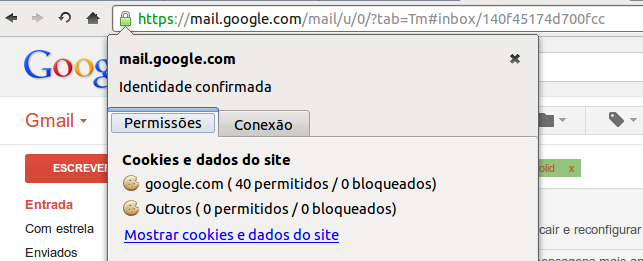
\includegraphics[scale=0.4]{img/gmail-ssl.png}
    \caption{SSL do Gmail}
\end{figure}

\end{frame}

\begin{frame}\frametitle{Acesso seguro através da internet}

SSL é uma nova camada de protocolo que opera em cima do protocolo TCP.

Permite ambas as máquina, cliente e servidor, estabelecer uma conexão
criptografada.

\end{frame}

\begin{frame}[fragile]\frametitle{Acesso seguro através da internet}

Entretanto isso é uma especificação, ou seja, alguém tem que
implementar. Algumas empresas que o implementam:

\begin{itemize}
\item
  OpenSSL (\href{openssl.org}{http://www.openssl.org/}) - Implementação
  livre e gratuita do SSL.
\item
  Apache-SSL (\href{apache-ssl.org}{http://www.apache-ssl.org/}) - um
  servidor web seguro, baseado no OpenSSL.
\item
  SSLeay (\url{ftp://ftp.uni-mainz.de/pub/internet/security/ssl/SSL/}) -
  uma implementação gratuita do Netscape's Secure Socket Layer.
\item
  Planet SSL
  (\url{http://www.rsasecurity.com/standards/ssl/developers.html}) -
  provê SSL para programas em C e Java.
\end{itemize}
\end{frame}

\begin{frame}[fragile]\frametitle{Acesso seguro através da internet}

Exemplo de mesma implementação para problemas diferentes:

multiplicação de 2 números:

\begin{verbatim}
2 * 3
\end{verbatim}
ou

\begin{verbatim}
2 + 2 + 2
\end{verbatim}
\end{frame}

\begin{frame}\frametitle{}

\slidetitle{Software Livre é seguro?}

\end{frame}

\begin{frame}\frametitle{Software Livre é seguro?}

\begin{figure}
    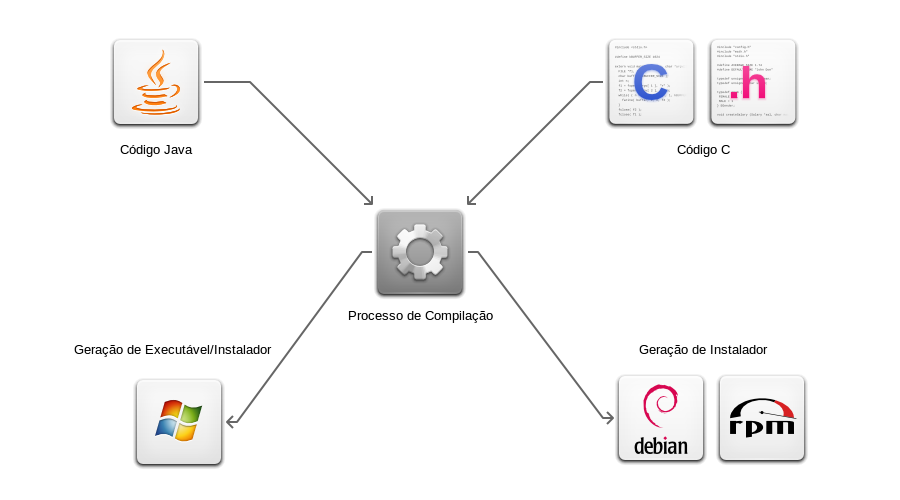
\includegraphics[scale=0.35]{img/codigos-compilados.png}
    \caption{Códigos Compilados}
\end{figure}

\end{frame}

\begin{frame}\frametitle{Software Livre é seguro?}

\begin{figure}
    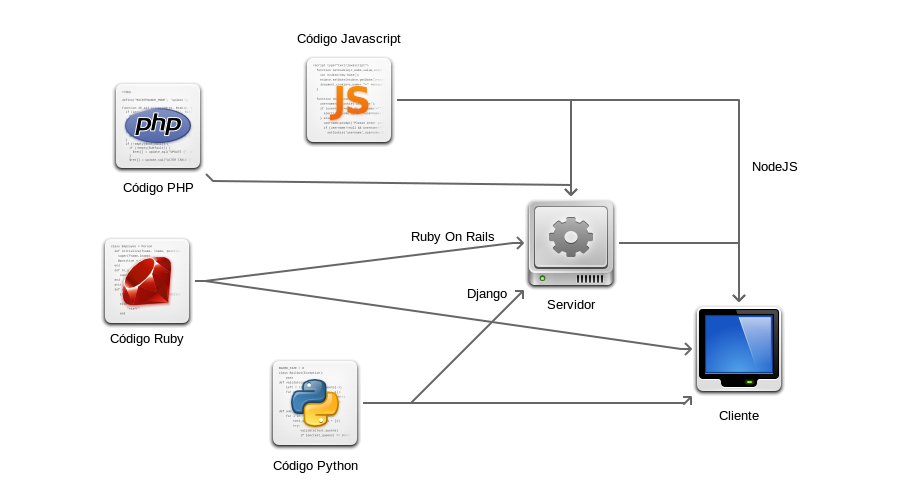
\includegraphics[scale=0.36]{img/codigos-interpretados.png}
    \caption{Códigos Interpretados}
\end{figure}

\end{frame}

\begin{frame}\frametitle{}

\slidetitle{O quão é seguro uma criptografia usando SSL?}

\end{frame}

\begin{frame}[fragile]\frametitle{}

\slidesubtitle{Levaria um tempo significativamente maior que a idade do universo para quebrar uma chave de 128-bits.}

Estima-se um pouco mais de 13 bilhões de anos.

Fonte: \url{http://www.inet2000.com/public/encryption.htm}

\url{http://www.digicert.com/TimeTravel/math.htm}

\end{frame}

\begin{frame}\frametitle{}

\slidetitle{Hackers e Crackers}

\end{frame}

\section{Hackers e Crackers}

\begin{frame}\frametitle{Hackers e Crackers}

Crackers são pessoas que invadem computadores com propósitos criminais
ou ganho pessoal.

Enquanto Hackers podem ser especialistas em segurança contratados por
empresas, com o objetivo de conhecer as vulnerabilidades e saná-las.

\end{frame}

\subsection{Hackeando Google e Duck Duck Go}

\begin{frame}[fragile]\frametitle{Hackeando Google}

Se hackear é uma coisa boa, então alguns sites permitem que isso seja
feito de forma a otimizar processos, como uma busca. Vejamos um exemplo
com o Google quando fazemos a busca:

\begin{verbatim}
comsolid filetype:pdf
\end{verbatim}
Além de buscar a palavra \emph{comsolid}, ele busca apenas arquivos pdf.

\end{frame}

\begin{frame}[fragile]\frametitle{Hackeando Google}

Ou ainda podemos fazer buscas em determinados sites somente. Basta fazer
uma busca na forma:

\begin{verbatim}
inkscape site:comsolid.org
\end{verbatim}
Essa busca pesquisa a palavra \emph{inkscape} no site comsolid.org

\end{frame}

\begin{frame}[fragile]\frametitle{Hackeando Duck Duck Go}

Duck Duck Go é um motor de busca preocupado com a pesquisa em si e a
privacidade.

\url{https://duckduckgo.com/}

Possui parte de seu código livre, isso inclui plugins, add-ons, etc.
Página do github

\url{https://github.com/duckduckgo/}

\end{frame}

\begin{frame}\frametitle{Hackeando Duck Duck Go}

Duck Duck Go permite \emph{hacks} mais engenhosos. Vamos a eles:

\begin{itemize}
\item
  !google comsolid
\item
  expand http://va.mu/dIwg
\item
  hello world python
\item
  ip address
\item
  github latexila
\item
  @comsolid
\item
  61900
\item
  age of linus torvalds
\item
  define free software
\item
  reverse dilosmoc
\end{itemize}
\end{frame}

\begin{frame}[fragile]\frametitle{Hackeando Duck Duck Go}

Temos ainda o \url{http://duckduckhack.com/}

\begin{figure}
    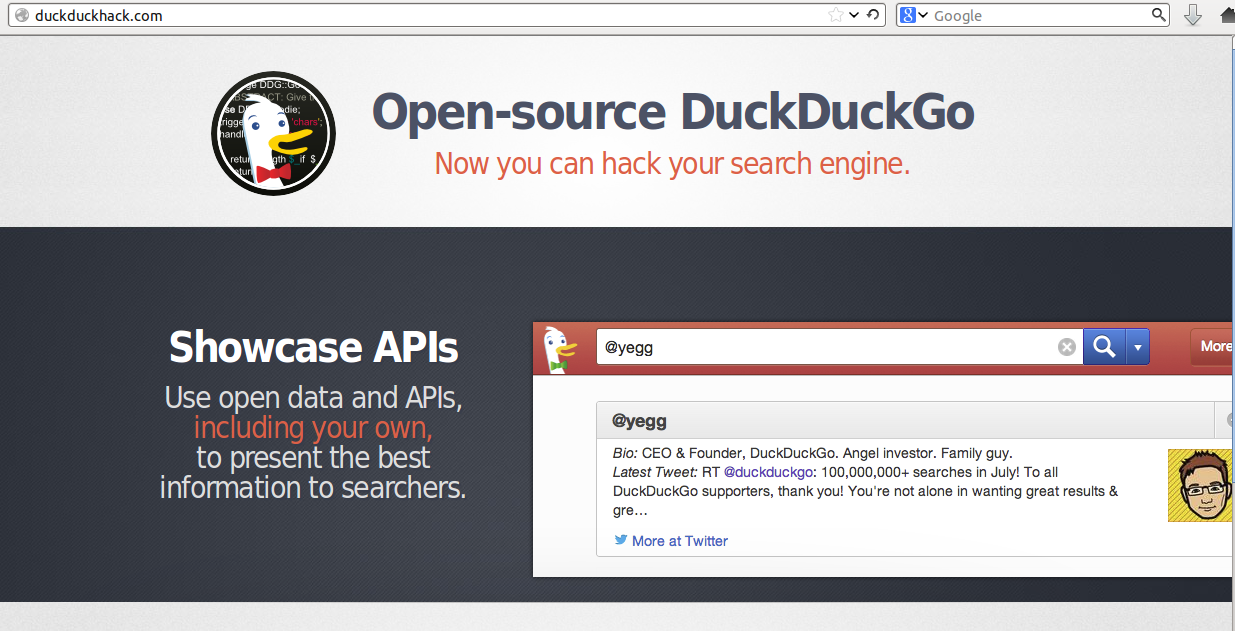
\includegraphics[scale=0.25]{img/duckduckhack.png}
    \caption{Duck Duck Hack}
\end{figure}

\end{frame}

\subsection{Técnicas para quebrar senhas}

\begin{frame}[fragile]\frametitle{Técnicas para quebrar senhas}

A técnica mais conhecida e natural é a força bruta, ou seja, tentar
todas as combinações possíveis até encontrar. Isso funciona até certo
ponto, quando a entrada é pequena.

Num artigo escrito por Dan Goodin no site \url{http://arstechnica.com}
em que descreve como Kevin Young, um pesquisador de segurança de senhas,
procedeu para descriptografar senhas vazadas pelo Antisec de uma empresa
chamada Stratfor.

\end{frame}

\begin{frame}[fragile]\frametitle{Técnicas para quebrar senhas}

Após quebrar 60\% das senhas usando listas de senhas disponíveis em:

\begin{itemize}
\item
  Hashcat - \url{http://hashcat.net/oclhashcat-plus/}
\item
  John the Ripper - \url{http://www.openwall.com/john/}
\end{itemize}
Para os outros 40\% ele ficou ``sem palavras'', então onde encontrá-las?

Que tal Wikipedia, Youtube, Bíblia, Projeto Gutenberg?

\end{frame}

\begin{frame}[fragile]\frametitle{Técnicas para quebrar senhas}

Uma das senhas era ``crotalus atrox'', nome científico de uma cobra. Tal
senha foi quebrada graças a esta página da Wikipedia:
\url{https://en.wikipedia.org/wiki/Crotalus_atrox}

Em seguida outras senhas fortes por serem grandes foram encontradas
como:

\begin{itemize}
\item
  ``from genesis to revelations'' (26)
\item
  ``I cant remember anything'' (24)
\item
  ``thereisnofatebutwhatwemake'' (26)
\item
  ``givemelibertyorgivemedeath'' (26)
\end{itemize}
\end{frame}

\subsection{Vazamento de senhas ao Linkedin}

\begin{frame}[fragile]\frametitle{Vazamento de senhas ao Linkedin}

Em Junho de 2012 um usuário anônimo postou no site
\url{http://insidepro.com/} uma lista com 6.5 milhões de hashs únicos
referentes a senhas pedindo ajuda para recuperá-las.

Após quebrar muitas das senhas descobriu-se que se tratava de um banco
de senhas do site Linkedin. Essa descoberta foi possível pelo número de
senhas com a palavra \emph{linkedin}.

\end{frame}

\begin{frame}[fragile]\frametitle{Vazamento de senhas ao Linkedin}

Na lista existiam:

\begin{itemize}
\item
  1 - linkedin (4408)
\item
  2 - link (2638)
\item
  3 - linked (2135)
\end{itemize}
Outras senhas encontradas:

\begin{itemize}
\item
  8 - love (1018)
\item
  11 - password (856)
\item
  16 - abc (750)
\end{itemize}
Mais informações em:
\url{http://www.ma.rhul.ac.uk/static/techrep/2013/MA-2013-07.pdf}

\end{frame}

\subsection{Engenharia reversa em firmware D-Link}

\begin{frame}[fragile]\frametitle{Engenharia reversa em firmware D-Link}

Todos sabemos que a D-Link é especializada em fazer roteadores, e eles
são um bom local para \emph{backdoors}. E isso foi exatamente que Craig
Heffner autor no blog \url{http://www.devttys0.com} encontrou.

Ele encontrou a partir de uma engenharia reversa no firmware de uma dos
roteadores.

\end{frame}

\begin{frame}[fragile]\frametitle{Engenharia reversa em firmware D-Link}

Após notar que certa função chamada \texttt{alpha\_auth\_check} soava
suspeita, ele foi saber o que exatamente ela fazia. Após um tempo ele
chegou no seguinte trecho de código:

\inputccodefile{ src/d-link.c }

\end{frame}

\begin{frame}\frametitle{Engenharia reversa em firmware D-Link}

Baseado no código fonte das páginas HTML e outros detalhes é sensato
concluir que os seguintes modelos são afetados:

\begin{itemize}
\item
  DIR-100
\item
  DIR-120
\item
  DI-624S
\item
  DI-524UP
\item
  DI-604S
\item
  DI-604UP
\item
  DI-604+
\item
  TM-G5240
\end{itemize}
\end{frame}

\begin{frame}[fragile]\frametitle{Engenharia reversa em firmware D-Link}

Quem quiser fazer um teste real existe um código em Python escrito pelo
próprio Craig e pode ser encontrado em:

\url{http://pastebin.com/vbiG42VD}

\inputpycodefile{ src/trecho-backdoor.py }

\end{frame}

\begin{frame}\frametitle{}

\slidetitle{Ataque ao Kernel}

\end{frame}

\subsection{Ataque ao Kernel}

\begin{frame}[fragile]\frametitle{Ataque ao Kernel}

\url{http://linux.slashdot.org/story/13/10/09/1551240/the-linux-backdoor-attempt-of-2003}

Em 2003, houve uma tentativa de backdoor no Kernel do Linux.

\inputccodefile{ src/backdoor.c }

Bastava chamar a função \texttt{wait4} e você viraria \emph{root}.

\end{frame}

\begin{frame}\frametitle{Ataque ao Kernel}

Comparemos os códigos original e o backdoor, e vejam se encontram a
diferença.

\inputccodefile{ src/original.c }

\inputccodefile{ src/backdoor.c }

\end{frame}

\section{Marco Civil da Internet no Brasil}

\begin{frame}\frametitle{Marco Civil da Internet no Brasil}

\textbf{O que é Marco Civil?}

É um projeto de Lei que visa estabelecer direitos e deveres na
utilização da Internet no Brasil. É a constituição da Internet no país.

\end{frame}

\begin{frame}\frametitle{Quais são os direitos e deveres?}

\begin{itemize}
\item
  \textbf{Neutralidade}: proíbe que provedores de internet discriminem
  certos serviços em detrimento de outros.
\item
  \textbf{Armazenamento de dados}: Operação de coleta de dados no Brasil
  deve respeitar a privacidade, proteção dos dados e sigilo das
  comunicações privadas.
\item
  \textbf{Retirada de conteúdo}: entidades que oferecem conteúdo e
  aplicações só serão responsabilizadas por danos gerados por terceiros
  se não acatarem ordem judicial exigindo a retirada dessas publicações.
\end{itemize}
\end{frame}

\begin{frame}[fragile]\frametitle{Quais são os direitos e deveres?}

\begin{itemize}
\item
  \textbf{Fim do marketing dirigido}: as empresas de acesso não poderão
  ``espiar'' o conteúdo das informações trocadas pelos usuários na rede.
  Há interesse em fazer isso com fins comerciais, como para publicidade.
\item
  \textbf{Sigilo e privacidade}: Provedores de acesso à internet serão
  obrigados a guardar os registros das horas de acesso e do fim da
  conexão dos usuários pelo prazo de seis meses, mas isso deve ser feito
  em ambiente controlado.
\end{itemize}
Para mais detalhes:
\url{http://www.molon1313.com.br/marco-civil-da-internet/}

\end{frame}

\begin{frame}\frametitle{Onde encontrar essa palestra?}

\begin{center}
Você pode baixar essa palestra e ainda outras em:

\bigskip

\large{\url{http://sige.comsolid.org/u/atilacamurca}}
\end{center}

\end{frame}

\begin{frame}\frametitle{}

\slidetitle{Dúvidas?}

\end{frame}

\begin{frame}\frametitle{Conecte-se}

\begin{center}
E-mail:\\
\texttt{camurca.home@gmail.com}

\medskip

Twitter:\\
\url{http://twitter.com/\#!/atilacamurca}

\medskip

Blog MAD3 Linux:\\
\url{http://www.mad3linux.org}

\medskip

COMSOLiD:\\
\url{http://comsolid.org/}\\
\url{http://twitter.com/\#!/comsolid}\\
\url{https://www.facebook.com/comsolid}

\medskip

Github:\\
\url{https://www.github.com/atilacamurca}
\end{center}

\end{frame}


\end{document}
